 \documentclass{article}
\usepackage[francais]{babel}
\def\printlandscape{\special{landscape}}    
\usepackage{amsmath}
\usepackage[utf8]{inputenc}
\usepackage[T1]{fontenc} 
\usepackage{fancybox} 
\usepackage{alltt}
\usepackage{graphicx}
\usepackage{lmodern}
\usepackage[colorlinks,hyperindex,bookmarks,linkcolor=blue,citecolor=blue,urlcolor=blue]{hyperref}
\usepackage{epsf}
\usepackage{enumitem}
\usepackage{pifont}
\usepackage{hyperref}
\usepackage{authblk}
\usepackage{titling}
\usepackage{floatflt}
\usepackage{changepage}
\usepackage[margin=0.5in]{geometry}
\usepackage{parskip}
\usepackage{subfig}
\setlength{\parindent}{30pt}

\begin{document}
\begin{center}
{\huge \textbf{Rapport de Début de Projet}}
\end{center}

\begin{center}
Participants : \textit{Baudet Léo-Paul / Miniaou Lucie / Tournier Pauline / Nguyen Mathieu\\}

\end{center}
\vspace{0.05\textheight}
\begin{center}
{\LARGE \textbf{Contrôle Magnétique d'Interface Liquides}}
\end{center}

\section{Présentation du Sujet}
Dans ce projet, nous allons étudier la forme d'un liquide déformé par un \textbf{champ magnétique}. Cette déformation est basée sur le principe de \textbf{lévitation magnétique}.
\newline
On considère au départ un récipient rempli d'un \textbf{liquide paramagnétique}, c'est-à-dire un liquide qui ne produit pas mais qui peut être sous l'effet d'un champ magnétique. Si on ne considère aucun champ au départ, alors le liquide est considéré comme étant en \textbf{équilibre hydrostatique}, seulement impacté par la gravité. Cependant si on ajoute à ce problème un champ magnétique, alors cette gravité est remplacée par une \textit{gravité effective} qui n'est pas forcément la même en tout cas de la surface considérée. 
\newline
Notre but est donc là de prédire la forme du liquide obtenue en fonction du champ magnétique à l'aide de \textbf{résolutions numériques}. On l'étudiera dans un premier temps d'un point de vue théorique, puis on instaurera notre méthode de calcul de manière numérique.

\section{Démarche à Aborder}
Afin de prédire les formes que peut avoir l'interface, il nous faut déterminer une équation donnant la \textbf{hauteur en fonction du champ magnétique H et de la position dans le milieu}, autrement dit une équation de type \textit{$\eta$(x,H)}. Il faut également prendre en compte d'autres facteurs comme les \textbf{ménisques} qui jouent également un rôle dans notre équation (étant donné que celles-ci influent sur la loi hydrostatique et donc la \textit{pression}). Notre objectif ici est donc de déterminer cette équation et de l'étudier, pour enfin la résoudre de manière numérique et prédire la forme obtenue en fonction du champ.
\section{Travail Réalisé Jusqu'a Présent}
Les ménisques cités précédemment influent sur la pression et leur courbure $K$ se détermine grâce à la tension d'interface $\gamma$ grâce à la formule suivante :
\begin{equation}
\kappa= \frac{\eta\prime\prime}{(1+\eta^{2}\prime)^{\frac{3}{2}}}
\label{eq01}
\end{equation}
De cette manière, étant donné que cette courbure influe sur la pression du milieu, on peut écrire les relations suivantes :
\begin{equation}
\kappa\eta = P_{\kappa} - P_{0} \indent \indent 
P_{\kappa} = -\rho gz- E_{fmag}
\label{eq02}
\end{equation}
Au final, en effectuant une coupe de la situation dans le repère (x,z), nous obtenons la relation suivante : 
\begin{equation}
\frac{\gamma n\prime\prime}{(1+\eta^{2}\prime)^{\frac{3}{2}}} + (\rho_{1} - \rho_{2})g\eta + \frac{1}{2}(\chi_{1} - \chi_{2})H^{2}(x,\eta)=0
\label{eq03}
\end{equation}
Avec $\eta$ = la hauteur, $\eta\prime$ = la pente, $\eta\prime\prime$ = la courbure 
\newline
Cette équation étant très compliquée, nous nous sommes séparés en deux groupes afin de discerner plusieurs cas sur lequel on peut s'attarder.
\newline
Etant donné que nous avons une équation différentielle \textbf{non linéaire}. Nous avons commencé par étudier des \textit{cas simples}.  Lucie et Pauline se sont penchés sur le cas où H = 0, tandis que Leo-Paul et Mathieu se concentre sur le cas ou $\gamma$ = 0. \\
\newline
- \underline{H = 0 :} lorsque $\eta\prime$ est très petit, on peut approcher le terme $\frac{\eta\prime\prime}{(1+\eta^{2}\prime)^{\frac{3}{2}}} = \eta\prime\prime$. On a donc la une équation différentielle de second degré classique avec deux constantes $\alpha$ et $\beta$ à déterminer. En utilisant la relation :
\begin{equation}
cos(\Theta) = \frac{\gamma_{SG}-\gamma_{LS}}{\gamma_{LG}}
\label{eq04}
\end{equation}
Nous avons pu déterminer une constante $\eta_{0}$ :
\begin{equation}
\eta_{0} = \frac{2\gamma cos(\Theta)}{\rho g}\frac{1}{R}
\label{eq05}
\end{equation}
Nous avons émis l'hypothèse qu'un ménisque est \textbf{symétrique d'un bout à l'autre du récipient}, nous avons donc considéré que les conditions limites étaient les mêmes en $\eta(0)$ et $\eta(d)$, ce qui nous a permis de déterminer les constantes $\alpha$ et $\beta$. 

Cependant, cette hypothèse n'étant pas forcément valide nous avons décidé d'utiliser une autre approche en s'aidant des conditions limites de la \textit{pente $\eta\prime(0)$}  et de $\eta(0)$. Cela nous a permis de trouver de nouveau  les constantes $\alpha$ et $\beta$. 
\newline
Nous avons ensuite programmé en C afin d'obtenir les valeurs numériques des constantes pour enfin tracer la fonction de la hauteur du liquide.
\begin{figure}[h]
	\centering
    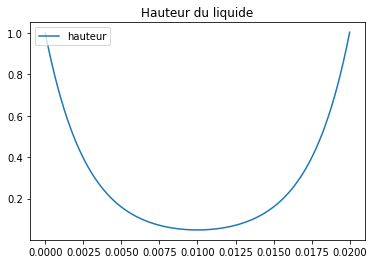
\includegraphics[width=.5\linewidth]{hauteur_fluide_eau.png}
    
\end{figure}
\newline\newline
- \underline{$\gamma$ = 0 :} L'équation simplifiée est maintenant :
\begin{equation}
(\rho_{1} - \rho_{2})g\eta + \frac{1}{2}(\chi_{1} - \chi_{2})H^{2}(x,\eta)=0
\label{eq06}
\end{equation}
Nous avons cherché à remplacer H par des \textbf{formules connues de champ magnétique}, comme par exemple pour un \textit{cylindre ou un fil infini}, mais il faut prendre en compte qu'un champ magnétique se calcule : 
\begin{equation}
\frac{B}{H} = \mu = \mu_{0}(1+ \chi_{m})
\label{eq07}
\end{equation}
Cependant, ce ne sont que des cas spécifiques, et pour résoudre cette équation pour un cas général, il nous faut là également utiliser des méthodes de résolutions numériques (dichotomie, Newton, Point Fixe...).
\newline
On a commencé à être en place les résolutions numériques (dichotomie et Point Fixe), et vérifier que ces méthodes peuvent être utilisées sur la fonction étudiée. On a aussi cherché à insérer les différents champs spécifiques dans notre équation pour y retrouver une fonction permettant de retrouver la hauteur. Il faut cependant passer des coordonnées cylindriques à la situation simplifiée que l'on a actuellement.

\section{Travail de Mathieu et Léo-Paul}
Léo-Paul s'est assuré dans un premier temps que les différentes méthodes de résolution numérique étaient applicables sur notre équation, notamment la méthode de Nexton. Pour cette méthode, il faut vérifier que la dérivée ne s'annule pas, peu importe le x. Une fois que cela est fait, il a pu implémenter toutes les méthodes de résolution, à savoir \textbf{la dichotomie, le point fixe de Picard et la méthode de Newton}.
\newline
Mathieu a commencé par implémenter les différents champs que l'on peut retrouver dans notre situation, plus spécialement les champs qui admettent \textbf{une invariance en y} (afin de n'avoir que x et z comme inconnues). On s'est finalement penché sur les 3 cas suivant : la nappe de courant, les deux fils à courant inversé et le dipole magnétique.
\newline
La nappe de courant est le champ le plus simple à mettre en place, car si on envoie le courant selon Oy, alors on n'a un \textbf{champ qui ne dépend que de z}. L'équation implémenté est la suivante : 

\begin{equation}
H(M) = \frac{jS}{2}\vec{u_{z}}
\label{eq08}
\end{equation}
\begin{figure}[h]
	\centering
    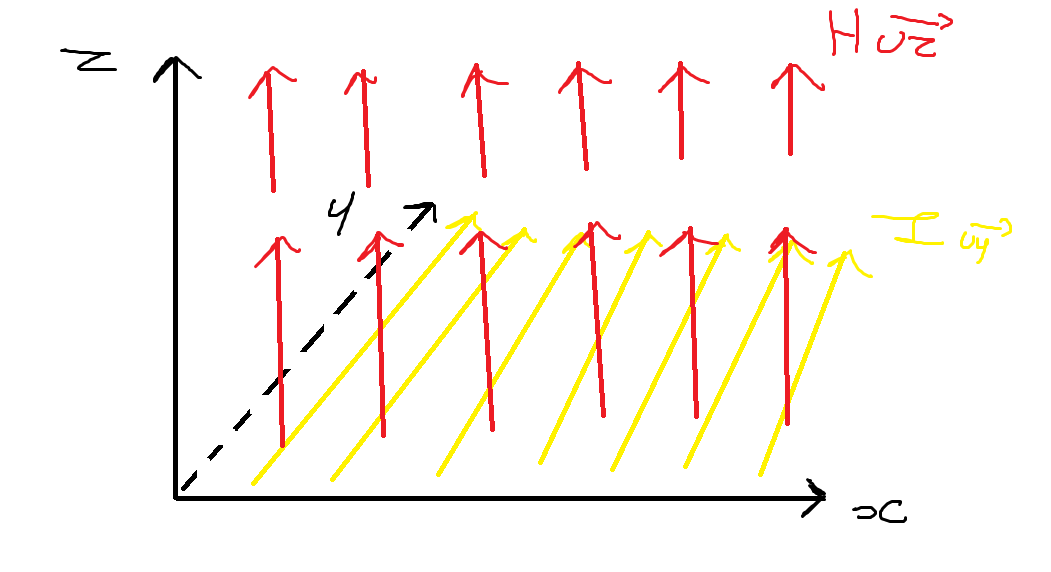
\includegraphics[width=.5\linewidth]{Nappe.png}
    
\end{figure}
\newpage

Les deux fils à courant sont plus complexes à définir, car leur champ est la plupart du temps donné dans des coordonnées cylindriques, et nous voulons les implémenter en coordonnées cartésiennes. Encore une fois, on fait en sorte d'avoir une \textbf{invariance en y}. Cela nous donne les formules suivantes :

\begin{equation}
H_{x}=\frac{-1}{\pi}pI\frac{2xz}{(x^2-y^2-p^2)^2+4x^2y^2} \indent\indent  H_{z}=\frac{-1}{\pi}pI\frac{x^2-y^2-p^2}{(x^2-y^2-p^2)^2+4x^2y^2}
\label{eq09}
\end{equation}
\begin{equation}
p = \sqrt{\frac{d^2}{4} - r^2} \indent\indent |H| = \sqrt{H_{x}^2+H_{z}^2}
\label{eq10}
\end{equation}
\begin{figure}[h]
	\centering
    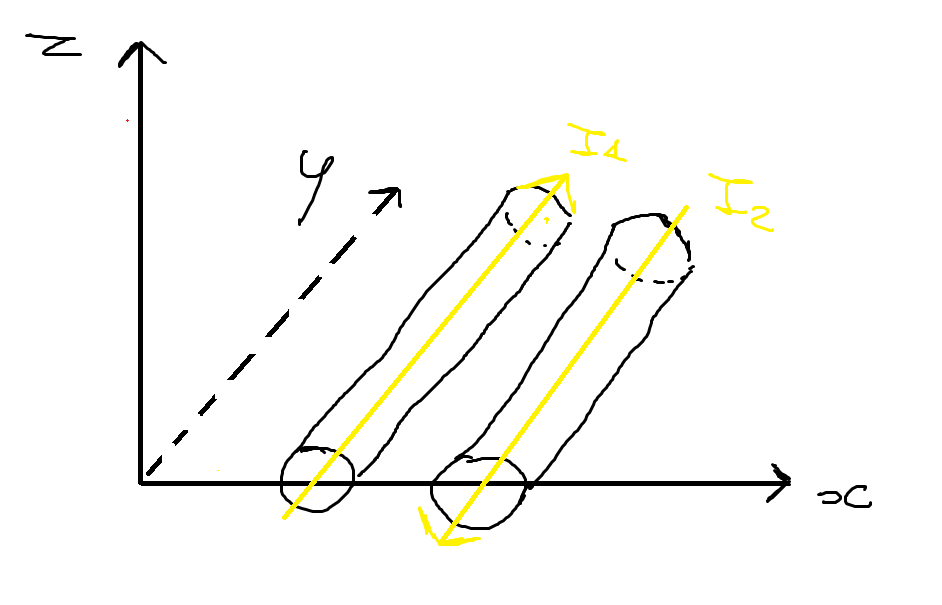
\includegraphics[width=.4\linewidth]{Fils.png}
    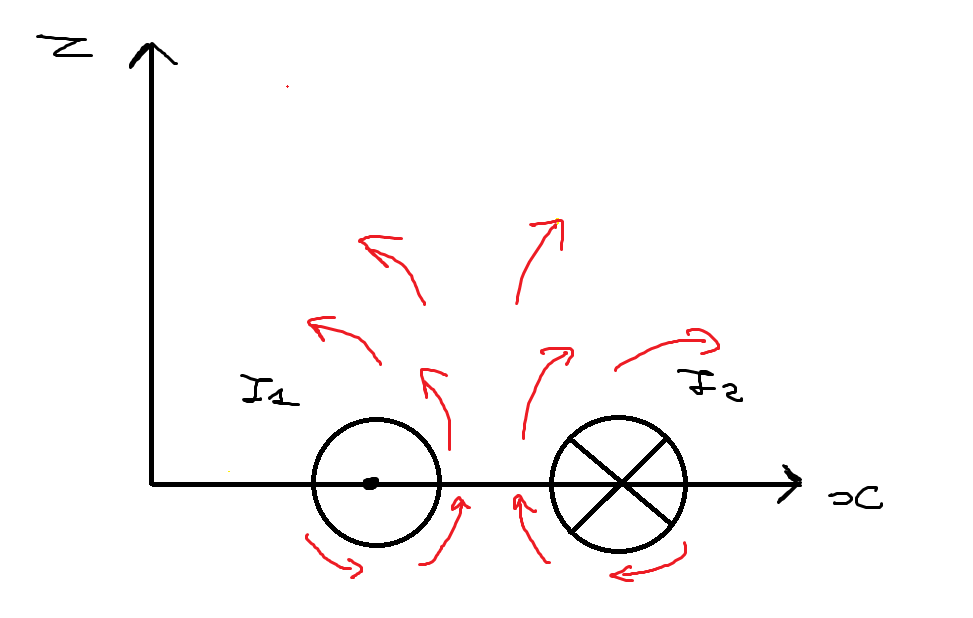
\includegraphics[width=.4\linewidth]{Fils2.png}
\end{figure}

Pour implémenter le dipôle magnétique, j'utilise la formule en carthésien suivante en considérant $m = IS$ :
\begin{equation}
H_{x} = \frac{m}{4\pi}\frac{3zx}{r^5}\indent\indent H_{y} = \frac{m}{4\pi}\frac{3zy}{r^5}\indent\indent H_{z}=\frac{m}{4\pi}\frac{1}{r^3}[\frac{3z^2}{r^2} - 1]
\end{equation}
En rappelant \textbf{$r = \sqrt{x^2 + y^2 +z^2}$}
\begin{figure}[h]
	\centering
    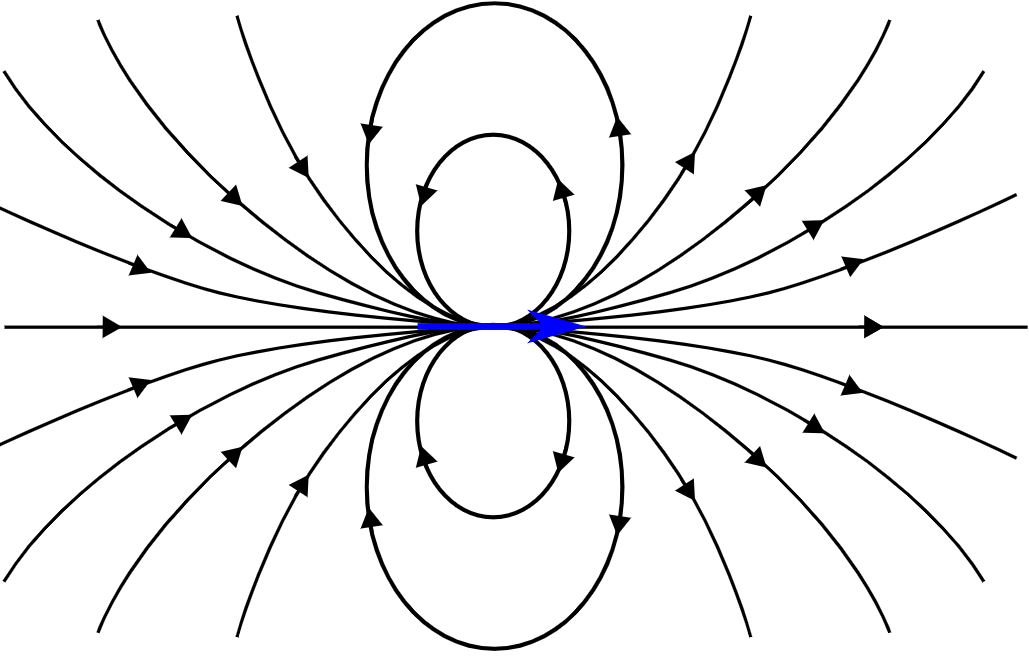
\includegraphics[width=.5\linewidth]{Dipole.png}
    
\end{figure}
\end{document}
   